\section{Software suite}
\label{app:dnn:software-suite}
The software used for the development of the DNN is based on industry-standard open-source ML libraries.
The entire workflow is based on Docker images~\cite{merkel2014docker} that provide the necessary packages that are all built with a Python~\cite{10.5555/1593511} frontend. The simulated MC samples provided centrally within the ATLAS collaboration are first transformed in order to remove the ATLAS software dependencies and make them easily useable with open-source ML libraries. The data are then stored in hdf5~\cite{fortner1998hdf} format, and handled with the numpy~\cite{2020NumPy-Array} and pandas~\cite{mckinney2010data} packages. The training is performed using Keras~\cite{chollet2015keras} and TensorFlow~\cite{abadi2016tensorflow} with the majority of the frontend provided by the FreeForestML~\cite{FreeForestML} library.
The scikit-learn~\cite{pedregosa2011scikit} library is used for data preprocessing, and the matplotlib~\cite{hunter2007matplotlib} package as well as the uhepp~\cite{UheppFrank} package are used for data visualization. The final DNN model is stored in JSON~\cite{pezoa2016foundations} format and deployed in the \HWW\ analysis using the C++ based LightWeight Tagger Neural Network (lwtnn)~\cite{daniel_hay_guest_2019_3249317} package.

\section{Optimization studies}
\label{app:dnn:opt-studies}
Several optimization studies for the VBF DNN were performed during the course of the author's PhD studies.
The following studies were performed with an earlier version of the DNN training setup, including an earlier version of the training data. For this reason, the absolute values of $Z0_{\mathrm{VBF}}$ (\cref{eq:significance-performance-metric}) are not necessarily comparable with other results presented in this thesis. However, the conclusions hold because the results were compared against each other.

\subsection{Study of DNN input variables}
Many sets of observables were studied for use as DNN input variables.
As baseline, the set of variables that was used in the BDT-based analysis of the previous iteration of the \HWW\ measurement \cite{HIGG-2016-07} is chosen, comprising in total 8 variables.
The performances of DNN models using a different number of variables are shown in \cref{tab:input-var-opt}.
Comparing the baseline to the results labelled ``S1'' shows significant improvements. This is an indication that the DNN exploits the correlations between the single $m_{\ell_\alpha j_\beta}$ (with $\alpha, \beta = 1, 2$) and other observables.
Although the discrimination power of \pTjone and \pTjtwo in linear dimension is limited, they also introduce a significant performance improvement when being included (``S2''). The same is true for the \pTjthree observable (``S3''), which adds information about whether a third jet is present in the event.
The final variable that was added and showed improvements is \METSig (``S4''). This observable has only recently been developed for use in the ATLAS collaboration \cite{ATLAS-CONF-2018-038} and is a strong discriminant between events with real undetected high-\pT particles and events where the \MET is the result of resolution effects.
Overall, the significance \ZVBF improves by a maximum of almost 50\% when comparing the baseline with the best performing set.
These results motivate the use of 15 input variables that correspond to the set labelled ``S4'' in \cref{tab:input-var-opt}.
In addition to the comparisons shown, several other observables were studied but did not lead to further improvements.
These tests included (i) using the $C_\ell$ observable separately instead of the sum for both leptons, $\lepetacent$, (ii) using \MET instead of \METSig, and (iii) using the \pT of both leptons on top of the other 15 variables.
Furthermore, the performance was studied of DNN models trained with all 15 variables except one. It was seen, that all chosen 15 variables provide discrimination power, although dropping highly correlated observables such as \mjj and \dyjj did not show large performance losses.

The physics-motivated optimization of the input variables was followed by the rather technical optimization of the neural-network architecture.
The performances of different setups are shown in \cref{tab:architecture-opt}. All results are very comparable to each other. Among the best performing architectures, the one with the least layers is chosen, which corresponds to the architecture labelled ``A4''. The results were produced with the set of variables labelled ``S3'' in \cref{tab:input-var-opt}.

\begin{table}[h]
    \centering
    \small
    \begin{tabular}{ l l | r}
        \toprule
        Identifier & Input Variables                                                                                         & \ZVBF \\
        \midrule
        Baseline   & \mjj, \dyjj, \lepetacent, \dphill, \mll, \mT, \pttot, $\sum_{\alpha,\beta=1,2} m_{\ell_\alpha j_\beta}$ & 7.7           \\
        S1         & Baseline w/ separate \mlonejone, \mlonejtwo, \mltwojone, \mltwojtwo,                                    & 8.57          \\
        S2         & S1 + \pTjone, \pTjtwo                                                                                   & 9.55          \\
        S3         & S2 + \pTjthree                                                                                          & 10.92         \\
        S4         & S3 + \METSig                                                                                            & 11.5          \\
        \bottomrule
    \end{tabular}
    \caption[Performance comparison between DNN models trained with different sets of input variables.]{Comparison of the significance metric \ZVBF between DNN models trained with different sets of input variables. The metric is evaluated using the validation set of a 2-fold cross-validation procedure.}
    \label{tab:input-var-opt}
\end{table}

\begin{table}[h]
    \centering
    \small
    \begin{tabular}{ l l | r}
        \toprule
        Identifier & Hidden layers                      & \ZVBF \\
        \midrule
        A1         & {32, 16, 8}                        & 10.4          \\
        A2         & {64, 32, 24, 16, 8}                & 10.6          \\
        A3         & {128, 64, 32, 24, 16, 8}           & 10.7          \\
        A4         & {256, 128, 64, 32, 24, 16, 8}      & 10.8          \\
        A5         & {128, 128, 64, 64}                 & 10.5          \\
        A6         & {512, 256, 128, 64, 32, 24, 16, 8} & 10.8          \\
        \bottomrule
    \end{tabular}
    \caption[Performance comparison between DNN models trained with different architectures.]{Comparison of the significance metric \ZVBF for DNN models using different architectures. The metric is evaluated using the validation set of a 2-fold cross-validation procedure.}
    \label{tab:architecture-opt}
\end{table}


\subsection{Optimization of the EW~$WW$ training fraction}
\label{app:sec:ewww-sample-fraction-optimization}
In a previous iteration of the VBF, \HWW\ analysis it was found that theoretical uncertainties related to particular processes dominate the final measurement uncertainties. In particular EW~$WW$ processes that mimic the VBF signal signature contributed significantly in the DNN bin with the largest DNN output (referred to as highest DNN bin), which lead to large uncertainties.
This prompted a change in the training procedure that places more emphasis on suppressing the EW~$WW$ background by increasing the training fraction, $S_\mathrm{frac}$, of the EW~$WW$ sample in the training.
In addition, an adapted performance metric, \ZVBFunc, was introduced to take into account theoretical uncertainties on the different processes when comparing different DNN trainings.
For this metric, approximate uncertainties are assumed for each process, see \cref{tab:rough-uncertainties}, by studying the total systematic uncertainties on the expected number of events in the highest DNN bin. They are included in the calculation of $Z0(s, b, \sigma)$ (\cref{eq:simple-sign}) via the $\sigma$ parameter.

The results of this optimization of the VBF DNN are shown by means of the expected number of events in the highest DNN bin in \cref{fig:bkg-fractions}. The contributions for each process without and with an increased training fraction for the EW~$WW$ processes are displayed.
The goal of this optimization is to achieve approximately equal number of expected events in the highest DNN bin for the dominant background processes with large uncertainties (which are ggF, EW~$WW$, $WW$, and \ttbar, see \cref{tab:rough-uncertainties}).
This is expected to prove beneficial when combining the uncertainties in the statistical analysis, compared to a scenario where one of the backgrounds dominates.
Due to this change, the final measurement uncertainties of the VBF, \HWW\ production cross section were reduced by roughly 5\%. 

The details of this study that lead to the final choice of the EW~$WW$ training fraction are visualized in \cref{fig:ew-fraction-scan}. All significances indicated are calculated prior to the statistical analysis and correspond to the \ZVBF as described in \cref{subsec:performance-metrics} (with two different binnings) and \ZVBFunc as described above. 
It can be seen that the EW~$WW$ fraction of the total background in the highest DNN bin (blue points; right axis) decreases as the training fraction used for EW~$WW$ processes in the training is increased.
The training with an EW~$WW$ training fraction of 0.05 roughly results in the background fractions indicated in \cref{fig:bkg-fractions-a}. 
They lead to worse results in the final statistical analysis because of the large contribution of EW~$WW$ in the last bin. 
Instead, the EW~$WW$ training fraction was set to 0.12, as highlighted in \cref{fig:ew-fraction-scan}.
In the x-range [0.06-0.12], the significance metrics that do not take into account systematic uncertainties show a slight downward trend. The \ZVBFunc metric, on the other hand, shows a very subtle upward trend, indicating a benefit of suppressing the EW~$WW$ content.
While this metric does not cover all aspects that determine the final measurement uncertainties, it helps to select the model that performs better in the final statistical analysis and therefore provides an improved measure over the more simple metrics that do not account for theory uncertainties.

\begin{table}[h]
    \centering
    \small
    \begin{tabular}{ c  | c}
        \toprule
        Background sample  & $\sigma^\text{rel}_\text{approx}$ \\
        \midrule
        $H_{\mathrm{VBF}}$ & 0.3                               \\
        $H_{\mathrm{ggF}}$ & 0.5                               \\
        $t\bar{t}$         & 0.3                               \\
        $Wt$               & 0.5                               \\
        $WW$ (Strong)      & 0.3                               \\
        $WW$ (EW)          & 0.5                               \\
        $Z/\gamma*$        & 0.25                              \\
        $V\gamma$          & 1                                 \\
        Other $VV$         & 0.12                              \\
        \bottomrule
    \end{tabular}
    \caption[Relative systematic uncertainty assumed on the different processes for constructing the significance metric \ZVBFunc.]{Relative systematic uncertainty $\sigma^\text{rel}_\text{approx}$ assumed on the different processes for constructing the significance metric \ZVBFunc.}
    \label{tab:rough-uncertainties}
\end{table}

\begin{figure}[t]
    \subfloat[No optimized training fractions] {
        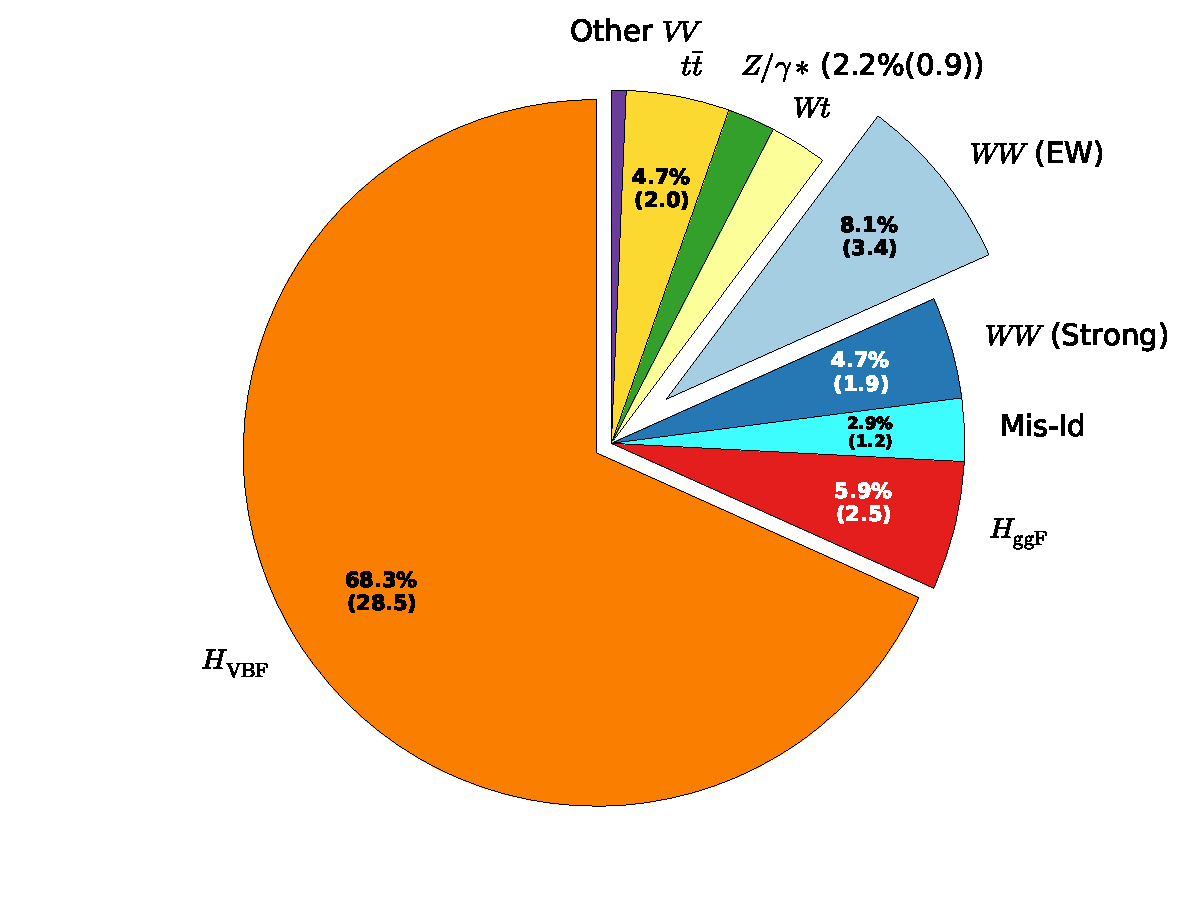
\includegraphics[width=0.49\textwidth,trim=35 0 0 0]{figures/plots/bkg-fraction-highest-bin/pie-chart-fractions-old.pdf}
        \label{fig:bkg-fractions-a}
    }
    \subfloat[Optimized EW~$WW$ training fractions] {
        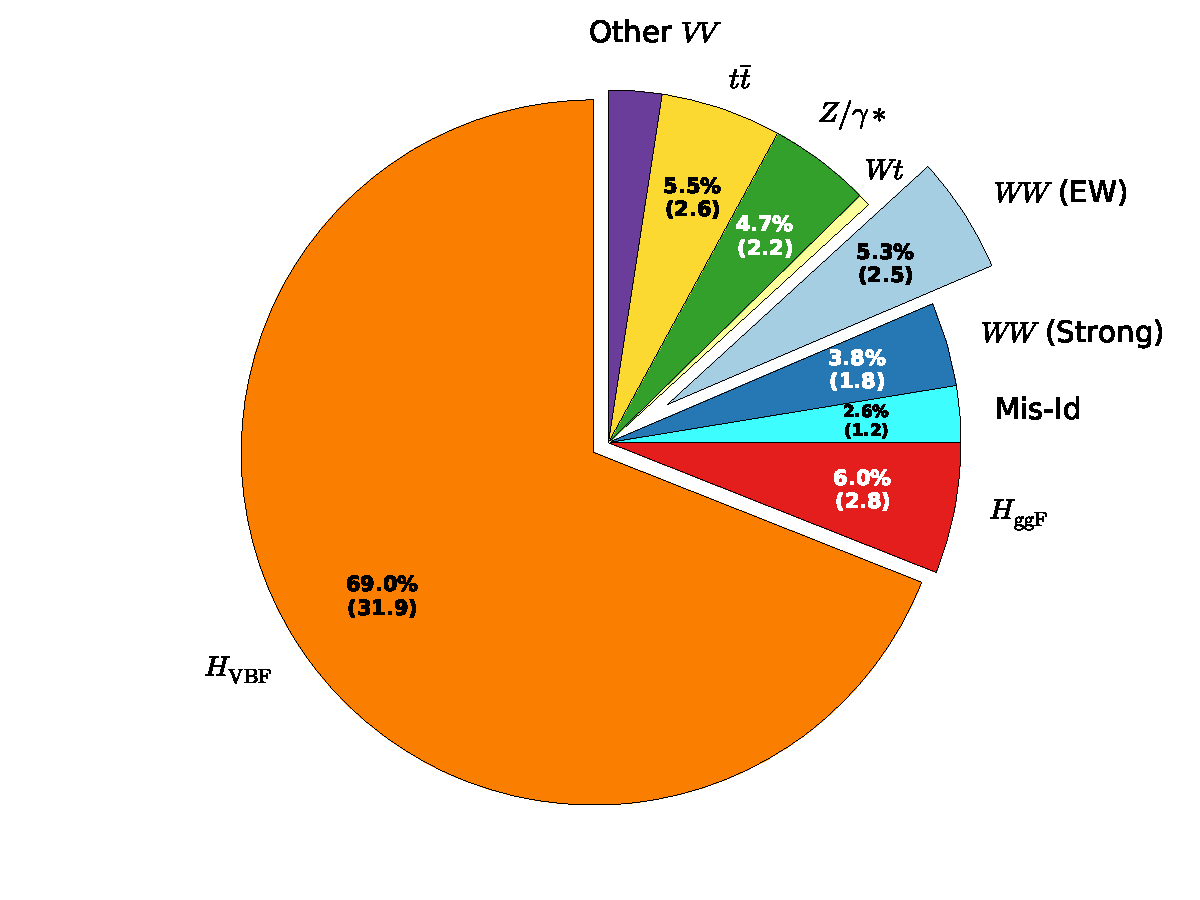
\includegraphics[width=0.49\textwidth,trim=35 0 0 0]{figures/plots/bkg-fraction-highest-bin/pie-chart-fractions-new.pdf}
        \label{fig:bkg-fractions-b}
    }
    \caption{Fraction of expected background events in the highest DNN output bin based on the validation set of a 5-fold cross-validation procedure for (a) default training fractions and (b) optimized EW~$WW$ training fraction.}
    \label{fig:bkg-fractions}
\end{figure}

% Plots made with SFUsMLKit on cedar with:
% ./plot.py -c configs/HWW/winningSubmission.cfg --trainingFolderName dropout-02-5-fold-aggressive-lr-schedule-2-fine-scan-ewww-scan-etafix/210805_9_0.12_8226149877761426764
\begin{figure}[t]
    % \subfloat[] {
    %     \newImageResizeCustom{0.47}{figures/plots/sample-fractions/sig_vs_lrate.pdf}
    % }
    % \subfloat[] {
    \newImageResizeCustom{0.6}{figures/plots/sample-fractions/sig_vs_ew_fraction_lr9.pdf}
    % }
    \caption{Significance metrics (left axis) and EW~$WW$ fraction of total background in the highest DNN output bin (right axis) for DNN models trained with different EW~$WW$ training fractions evaluated using the validation set of a 5-fold cross-validation procedure. The metric $\ZVBF$ (40 bins) is calculated as described in \cref{subsec:performance-metrics} and using 40 equidistant histogram bins. The metric $\ZVBF$ (var. bins) is calculated similarly but using a rebinned histogram according to the procedure outlined in \cref{subsec:performance-metrics}. The metric $\ZVBFunc$ (var. bins), other than the other ones, consider rough estimates of systematic uncertainties for the different processes, also using a rebinned histogram. The assumed uncertainties are shown in \cref{tab:rough-uncertainties}.}
    \label{fig:ew-fraction-scan}
\end{figure}
